\zag{Дисперсия света}

\subzag{Элементарная классическая теория} 

Хорошо известное наличие зависимости показателя преломления от частоты
падающего света представляет собой факт первостепенной важности.
Именно в этом вопросе феноменологическая электродинамика Максвелла
зашла в тупик. Явление дисперсии потребовало для своего объяснения
создания детализированной электронной теории. Во 2 главе была
установлена связь между показателем преломления (рефракцией) и
поляризуемостью атома или молекулы. Наличие дисперсии не нарушает
этой связи, но из факта зависимости показателя преломления от
длины волны следует, что сама поляризуемость является функцией
частоты света. Для понимания сущности явлений молекулярной оптики,
которые все, так или иначе, связаны с поляризуемостью, необходимо,
следовательно, нахождение вида зависимости поляризуемости от
частоты света, необходимо построение полной теории поляризуемости
с учетом дисперсионной зависимости.

Строгая молекулярная теория распространения света в веществе
изучает наложение вторичных световых волн, излучаемых молекулами,
возбужденными внешней электромагнитной световой волной. Эта теория
была разработана рядом авторов на основе представлений
кристаллооптики. Рассматривается плоская световая волна,
попадающая в изотропную среду. Под действием  поля волны $\vec E$
в молекулах среды индуцируются диполи, совершающие вынужденные
колебания с частотой, равной частоте световой волны. Эти диполи
являются источниками вторичных, на этот раз сферических световых
волн. Поле, действующее на данную молекулу
--- диполь $j$ слагается из внешнего поля $\vec E$ и полей
сферических волн, создаваемых остальными диполями:
$$\vec E'^{(j)}=\vec E+\sum_{l}E'^{(jl)}.\noq$$
В результате наложения первичной плоской волны и всех вторичных
волн, излучаемых всеми диполями среды, содержащей $N_1$ диполей в
единице объема, получается результирующая волна, которая, как
показывает расчет, является плоской. Внутри среды эта волна
распространяется в соответствии с законом преломления, вне ее ---
в соответствии с законом отражения.

В молекулярной теории, основывающейся на электронном рассмотрении,
волны, испускаемые диполями, распространяются от молекулы до
молекулы со скоростью света в вакууме $c$. Скоростью $c'={c\over
n}$ характеризуется лишь результирующая волна.

Весьма важным принципиальным результатом молекулярной теории
является отсутствие света по направлениям, отличным от направления
преломленного и отраженного лучей. Этот результат получается при
условии, что имеет место равномерное распределение вещества по
объему, и, следовательно, постоянное значение $N_1$. При этом
условии свет гасится по всем направлениям, кроме предписанных
законами волновой оптики, вследствие интерференции, так как
вторичные волны когерентны. Строгая теория приводит к соотношению:
$${n^2-1\over n^2+2}={4\pi\over3}N_1\alpha,$$
где $\alpha$ --- средняя поляризуемость молекул, причем постоянная
внутреннего поля ${4\pi\over3}$ получается, как непосредственное
следствие предполагаемой равномерности в распределении молекул.

Очевидно, что исследование дисперсии в рамках классической
волновой теории должно строиться на тех же основаниях. Поэтому мы
должны рассмотреть излучение и поглощение света элементарными
излучателями. Такими излучателями в электронной теории являются
электроны, совершающие гармонические колебания около положения
равновесия. Рассмотрим свободные колебания таких гармонических
осцилляторов. Они описываются уравнением движения:
$$m\ddot{\vec r}+k\vec r=0,\noq$$
где $m$ --- масса, $k$ --- упругая постоянная. Общее решение этого
уравнения имеет вид:
$$\vec r=\vec a\cos \omega_0t+\vec b\sin \omega_0t,\noq$$
где $$\omega_0=\sqrt{{k\over m}}.\noq$$ Колеблющийся электрон
имеет дипольный момент:
$$\vec p=e\vec r=e\vec a\cos \omega_0t+e\vec b\sin \omega_0t.\noq$$
Следовательно:
$$\ddot{\vec p}=-\omega_{0}^2\vec p.$$
В электродинамике доказывается, что поле нейтральной системы
зарядов на больших от нее расстояний совпадает в первом
приближении (при условии ${x_0\omega\over c}\ll 1$) с полем
диполя, момент которого равен моменту системы. Гармонический
осциллятор является источником сферических световых волн,
электрическая и магнитная напряженности которых выражаются в
волновой зоне (на расстояниях $R\gg x_0$) следующим образом:
$$\vec E={1\over c^2R^3}\left[\vec R\left[\vec R\ddot{\vec
p}\right]\right],\noq$$
$$\vec H=-{1\over c^2R^2}\left[\vec R\ddot{\vec
p\mathstrut}\right],\noq$$ откуда вектор Умова-Пойнтинга:
$$\vec S={c\over4\pi}[\vec E\vec H]={c\over4\pi}{1\over
c^{4}R^5}\vec R\left[\vec R\ddot{\vec p}\right]^2.\noq$$
Расположение векторов $\vec p$, $\vec E$, $\vec H$, $\vec R$ и
$\vec S$ показано на рис. 3.1. Интенсивность излучения по
некоторому направлению $\vec R$, составляющему угол $\vartheta$ с
направлением колебания осциллятора, выражается величиной:
$$|\vec S|={1\over 4\pi c^3R^2}\left(\ddot{\vec
p}\right)^2\sin^2\vartheta.\noq$$

\begin{figure}[tbp]
\centerline{\hbox{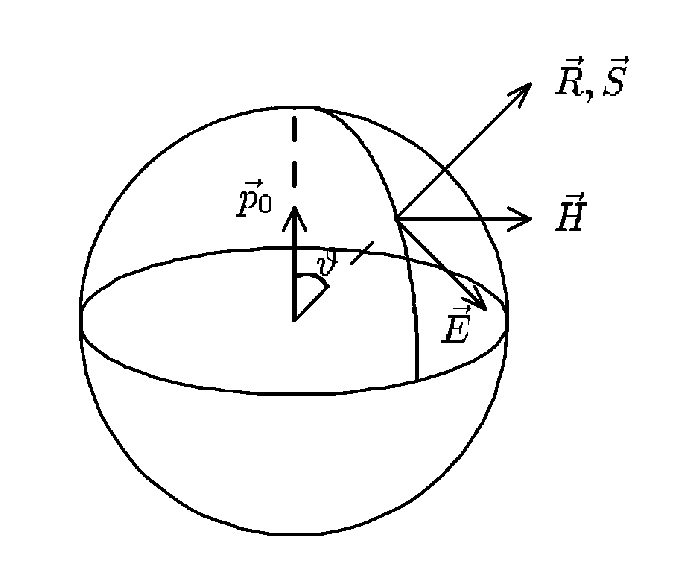
\includegraphics[scale=0.6]{Ris/ris_eps/ris3_01.eps}}}

\risp{1}{Излучение колеблющегося
диполя}
\end{figure}

Подставляя в \eqn{9} значение $
\ddot{\vec p}=-\omega^2_0\vec p$, находим:
$$|\vec S|={1\over4\pi c^3R^2}\omega^4_0\vec p^2\sin^2\vartheta.\eqno
(3.9a)$$ Общая энергия, излучаемая осциллятором в единицу времени,
есть интеграл от $|\vec S|$ по сферической поверхности:
$${dW\over dt}=\int\int|\vec S|R^2\sin\vartheta d\vartheta
d\varphi={2\over3}{\omega_0^4\over c^3}\overline{p^2}.\noq$$ Здесь
$\overline{p^2}$ --- среднее значение $p^2$ за данный промежуток
времени. В силу соотношений \eqn{5-7}, имеем:
$$\vec E={\omega_0^2\over c^2R^3}\left[\vec R\left[\vec p\vec
R\right]\right]=\vec E_1\cos \omega_0t+\vec E_2\sin
\omega_0t,\noq$$
$$\vec H={-\omega_0^2\over c^2R^3}\left[\vec p\vec
R\right]=\vec H_1\cos \omega_0t+\vec H_2\sin \omega_0t.\noq$$
Иными словами, сферическая волна, испускаемая гармоническим
осциллятором, есть монохроматическая волна с частотой $\omega_0$,
той же самой, с которой колеблется осциллятор. Однако, в силу
\eqn{10}, осциллятор не может колебаться по закону \eqn{2}, ибо он
не непрерывно отдает свою энергию в виде излучения, и его энергия
колебаний, в отсутствие внешней силы, их поддерживающей,
непрерывно уменьшается, --- колебания затухают.

Для того, чтобы удовлетворить закону сохранения энергии, мы должны
ввести в уравнение движения добавочную силу --- такую, чтобы ее
наличие определяло потерю энергии в соответствии с \eqn{10}.
Напишем:
$$m\ddot{\vec r}+k\vec r=\vec K,\noq$$
и после умножения на $\dot{\vec r}$:
$${d\over dt}\left({m\over2}\dot{\vec{r^2}}+{k\over2}\vec{r^2}\right)=\vec K\dot{\vec r}.$$
Здесь слева стоит изменение энергии ${dW\over dt}$ --- ее
уменьшение. Следовательно:
$$\overline{\vec K\dot{\vec r}}=-{2\omega_0^4\over3c^3}\overline{p^2}=
-{2e^2\over3c^3}\overline{\ddot{\vec{r^2}}},$$ и, так как
$${d\over dt}\left(\dot{\vec r}\ddot{\vec
r}\right)\equiv\ddot{\vec r^2}+\dot{\vec r}\tridot{\vec r},$$ имеем
среднее значение $\vec K\dot{\vec r}$ в интервале от $t=0$ до
$t=T$:
$$\overline{\vec K\dot{\vec
r}}={2e^2\over3c^3}\overline{\tridot{\vec r}\dot{\vec r}}-{2 e^2\over3c^3}
{\left( \dot{\vec r}\ddot{\vec r})_{t=T}-(\dot{\vec r}\ddot{\vec r})_{t=0}\right)\over T}$$
При больших $T$ второе слагаемое можно опустить:
$$\overline{\vec K\dot{\vec
r}}={2e^2\over3c^3}\overline{\tridot{\vec r}\dot{\vec r}}.  \noq$$

Мы удовлетворим нашим условиям в среднем, положив
$$\vec K={2e^2\over3c^3}\tridot{\vec r},\noq$$
и для почти периодических движений:
$$\vec K=-{2e^2\omega_0^2\over3c^3}\dot{\vec r}.\noq$$
Уравнение движения принимает вид:
$$m\ddot{\vec r}+m\gamma\dot{\vec r}+k\vec r=0,\noq$$
где
$$\gamma={2e^2\over3c^3m}.$$
Благодаря наличию члена $m\gamma\dot{\vec r}$, характеризующего
силу трения, амплитуда колебаний будет затухать. Получаем решение
\eqn{17}, аналогичное \eqn{3}, причем:
$$\vec a=\vec a_0e^{-\gamma/2t},\hskip 4mm \vec b=\vec
b_0e^{-\gamma/2t}.$$ Итак, решение \eqn{17} имеет вид:
$$\vec r=e^{-\gamma/2t}(\vec a_0\cos \omega_0t+\vec b_0\sin \omega_0t).\noq$$
Это решение, как легко видеть, удовлетворяет уравнению \eqn{13}
при малом затухании, т.е. в случае $\gamma\ll \omega_0$. Нетрудно
убедиться, что решение \eqn{18} соответствует потере энергии
\eqn{10}. Определив $\vec r$, как $\vec r=\vec Ae^{i\omega_0t}$,
где $\vec A$ --- комплексный вектор, напишем:
$$\vec p=e\vec r=\vec p_0e^{-\gamma/2t}e^{i\omega_0t},\noq$$
и, согласно \eqn{11}, \eqn{12},
\begin{plain}$$\eqalign{\vec E=&\vec E_0e^{-\gamma/2t}e^{i\omega_0t},\cr
\vec H=&\vec H_0e^{-\gamma/2t}e^{i\omega_0t}, }\noq$$\end{plain} где $p_0$,
$E_0$, $H_0$ --- комплексные амплитуды. Волна \eqn{20} уже не
является монохроматической, но характеризуется некоторым
распределением интенсивностей по частотам $\omega$. Чтобы найти
это распределение, разложим \eqn{20} в интеграл Фурье: \vskip -2mm
\begin{plain}$$\eqalign{
&\vec E={1\over2}\int\limits_{-\infty}^{+\infty}\vec
E(\omega)e^{i\omega t}d\omega, \cr &{\rm \hbox{где}} \cr &\vec
E(\omega)={1\over2\pi}\vec
E_0\int\limits_0^{+\infty}e^{i(\omega_0-\omega)t}e^{-\gamma/2t}dt
.} \noq$$\end{plain} Имеем: \vskip -2mm
$$\vec E(\omega)={1\over2\pi}\vec E_0{1\over i(\omega_0-\omega)-\gamma/2},$$
и распределение интенсивностей: \vskip -2mm
$$I(\omega)\cong|\vec E(\omega)|^2=I_0{\gamma\over2\pi}{1\over
(\omega_0-\omega)^2-(\gamma/2)^2},\noq$$ где $I_0$ ---
интегральная интенсивность, равная
$\int\limits_{-\infty}^{+\infty}I(\omega)d\omega$.

Вид кривой $I(\omega)$ представлен на рис. 3.2. Кривая имеет
максимум при $\omega=\omega_0$ (точнее, максимум слегка сдвинут
относительно $\omega_0$, но сдвигом можно пренебречь, так как
${\gamma\over \omega_0}\ll 1$). Мы можем охарактеризовать ширину
линии (полосы) излучения интервалом значений $\omega$, в котором
$I(\omega)$ имеет величину больше половины максимальной
$I(\omega_0)$, равной: \vskip -2mm
$$I(\omega_0)=I_0{2\over\pi\gamma}.$$

\begin{figure}[tbp]
\centerline{\hbox{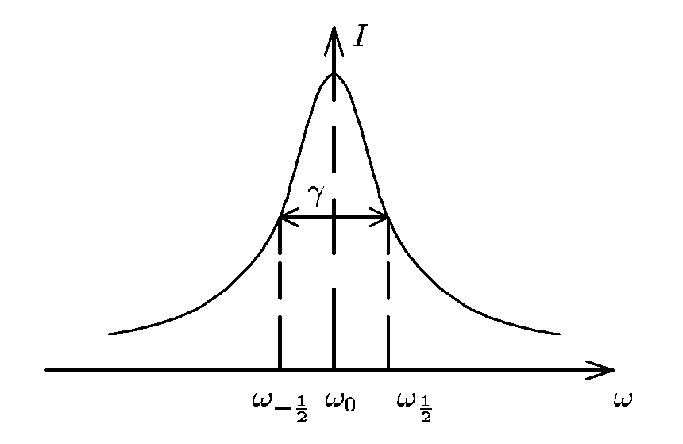
\includegraphics[scale=0.6]{Ris/ris_eps/ris3_02.eps}}}

\risp{2}{Контур спектральной линии} 
\end{figure}

Ищем значения $\omega$, при которых
$$I(\omega_{1\over2})={1\over2}I(\omega_0)=I_0{1\over\pi\gamma},$$
имеем:
$$\omega_{1\over2}=\omega_0\pm{\gamma\over2}.$$
Следовательно, полуширина спектральной линии, излучаемой
затухающим осциллятором, дается значением:
$$\Delta \omega=\gamma.\noq$$

Укажем, что затухание вследствие излучения и соответствующее
расширение спектральной линии обычно малы по сравнению с
затуханием и расширением, вызванными другими причинами:
соударениями между излучающими частицами, влиянием электрического
поля, явлением Доплера и т.д. Во всех этих случаях по-прежнему
применимо уравнение \eqn{17}.

Перейдем теперь к нашей непосредственной задаче, к рассмотрению
явления дисперсии. Рассмотрим электрон --- гармонический
осциллятор, находящийся под действием внешней световой волны.
Пренебрегая затуханием, мы напишем уравнение движения в виде:
$$m\ddot x+kx=eE_x,\noq$$
где $E_x$ --- напряженность поля световой волны, действующей на
электрон с зарядом $e$. Переходя сразу к дипольному моменту,
получим:
$$\ddot{\vec p}+\omega_0^2\vec p={e^2\over m}\vec E.\noq$$
Но поле $\vec E$ --- поле световой волны периодически зависит от
времени с частотой падающего света:
$$\vec E=\vec E_0e^{i\omega t}.\noq$$
Следовательно, уравнение \eqn{25} есть уравнение вынужденных
колебаний. Ищем его решение в виде:
$$\vec p=\vec p_0e^{i\omega t}.\noq$$
Подставляя в \eqn{25}, имеем:
$$\vec p(\omega_0^2-\omega^2)={e^2\over m}\vec E,$$
откуда:
$$\vec p={e^2\over m}{1\over \omega_0^2-\omega^2}\vec E=\alpha\vec E.\noq$$
Т.е. поляризуемость гармонического осциллятора зависит от частоты
внешнего поля по дисперсионному закону:
$$\alpha={e^2\over m}{1\over \omega_0^2-\omega^2}.\noq$$
В статическом поле $\omega=0$ и
$$\alpha={e^2\over m\omega_0^2}={e^2\over k}.\noq$$
Здесь мы говорим о некотором скалярном осцилляторе, колеблющемся в
том же направлении, что и $\vec E$, и, соответственно, о скалярной
поляризуемости $\alpha$. Очевидно, что подобное рассмотрение
применимо и к поведению среднего дипольного момента,
индуцированного полем.

В этих рассуждениях мы пренебрегли влиянием магнитного поля. В
теории дисперсии оно мало существенно. Но им нельзя пренебрегать в
тех случаях, когда мы рассматриваем действие сильного внешнего
магнитного поля. В этом случае вместо уравнения \eqn{24} напишем:
$$m\ddot x+kx=eE_x+{e\over c}\left[\dot{\vec r}\vec
H\right]_x.\eqno (3.24a)$$ Магнитное поле создает действующую на
электрон силу Лорентца. Здесь $\vec r=\vec r(x,y,z)$. При
одинаковых порядках величины $E$ и $H$ (поле световой волны),
магнитная сила много меньше электрической, ибо:
$${|\dot{\vec r}|\over c}\ll 1.$$
Согласно \eqn{29}, поляризуемость становится бесконечно большой,
когда частота внешнего поля совпадает с собственной частотой
осциллятора --- с той частотой, которую он сам излучает.

По основному закону спектроскопии --- закону Кирхгоффа -- эта
частота есть, тем самым, частота поглощения осциллятора.

Значение $\alpha\rightarrow\infty$ парадоксально и получилось
потому, что мы пренебрегли затуханием. Учтем это обстоятельство:
$$\ddot p+\gamma\dot p+\omega_0^2p={e^2\over m}E_0e^{i\omega t}.\noq$$
По-прежнему ищем решение в виде \eqn{27}. Получаем:
$$p=\alpha E={e^2\over m}{1\over \omega_0^2-\omega^2+i\omega\gamma}E.\noq$$
Мы получили комплексное выражение для поляризуемости. Для того,
чтобы раскрыть его смысл, вернемся к формуле Лорентц-Лоренца
\eqn{18}. Подставив в нее полученное выражение для $\alpha$,
имеем:
$${\tilde n^2-1\over\tilde n^2+2}={4\pi\over3}N_1\tilde\alpha = {4\pi\over3}N_1
{e^2\over m}{1\over \omega_0^2-\omega^2+i\omega\gamma},\noq$$ где
$\tilde n$ --- комплексный показатель преломления. Для газов:
$$\tilde n=1+2\pi N_1{e^2\over m}{1\over
\omega_0^2-\omega^2+i\omega\gamma}.\noq$$ Представим комплексный
показатель в виде:
$$\tilde n=n-i\chi.\noq$$
Результирующая плоская волна в среде --- преломленная волна ---
может быть представлена выражением:
$$E=E_0e^{i\omega\left(t-{\tilde n R\over
c}\right)}=E_0e^{-{\chi \omega R\over
c}}e^{i\omega\left(t-{nR\over c}\right)}.\noq$$ Таким образом,
мнимый член в $\tilde n$ характеризует затухание проходящей волны
по мере прохождения ею пути $R$. Коэффициент $\chi$ называется
коэффициентом экстинкции и выражает поглощение света в веществе.
Действительно, согласно уравнению \eqn{36}, интенсивность
проходящего света должна ослабляться в поглощающей среде по
закону:
\begin{plain}
$$\eqalign{I=&I_0e^{-kR},\cr
k=&2{\chi \omega\over c}.}\noq$$ Вычислим $n$ и $\chi$. Для газов
получаем, согласно \eqn{34}:
$$n-i\chi=1+2\pi N_1{e^2\over m}\left\{{\omega_0^2-\omega^2\over
(\omega_0^2-\omega^2)^2+\gamma^2\omega^2}-i{\gamma
\omega\over(\omega_0^2-\omega^2)^2+\gamma^2\omega^2}\right\},$$
откуда
$$\eqalign{n=&1+2\pi N_1{e^2\over m}{\omega_0^2-\omega^2\over
(\omega_0^2-\omega^2)^2+\gamma^2\omega^2},\cr \chi=&2\pi
N_1{e^2\over m}{\gamma
\omega\over(\omega_0^2-\omega^2)^2+\gamma^2\omega^2}.}$$ 
\end{plain}
Ход
$n(\omega)$ показан на рис. 3.3. Мы видим, что ход $\chi$ связан с
видом линии (полосы) поглощения, полуширина которой $\Delta
\omega=\gamma$. В области <<$\omega_0$>> --- аномальная дисперсия.

В области, удаленной от собственной частоты поглощения можно
пренебречь значением $\gamma^2\omega^2$ в знаменателе по сравнению
с $(\omega_0^2-\omega^2)$, и, на равных основаниях, пренебречь
мнимым членом в выражении поляризуемости. Здесь справедливо
выражение для поляризуемости \eqn{29}:
$$\alpha={e^2\over m}{1\over \omega_0^2-\omega^2}.$$

\begin{figure}[tbp]
\centerline{\hbox{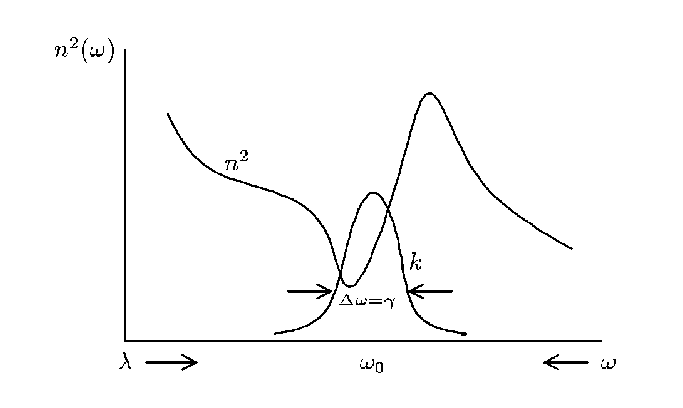
\includegraphics[scale=0.9]{Ris/ris_eps/ris3_03.eps}}}

\risp{3}{Кривая дисперсии}
\end{figure}

Однако реальная система --- атом, молекула, обладает не одной,
а целым набором собственных частот $\omega_0$, наблюдаемых в
спектре испускания или поглощения. С точки зрения классической
электронной теории, мы должны с каждой частотой сопоставить
некоторый гармонический осциллятор с зарядом и массой $e_i$,
$m_i$. Обозначим:
$${e_i^2\over m_i}=f_i{e^2\over m},$$
где $e$ и $m$ --- заряд и масса электрона. Поляризуемость всей
системы представится выражением:
$$\alpha={e^2\over m}\sum_{i}{f_i\over \omega_i^2-\omega^2},\noq$$
причем сумма всех $f_i$ должна равняться полному числу
осцилляторов-электронов в рассматриваемой системе:
$$\sum_{i}f_i=Z.\noq$$
Безразмерные величины $f_i$ называются силами осцилляторов, $f_i$
могут, конечно, быть нецелыми числами и, в частности, возможны
значения $f_i\ll 1$.

Очевидно, что $f_i$ характеризуют интенсивность линий (полос)
испускания и поглощения системы. В самом деле, при учете
затухания, согласно \eqn{34}:
$$\tilde n=1+2\pi N_1{e^2\over m}\sum_{i}{f_i\over
\omega_i^2-\omega^2+i\gamma_i \omega},$$ и для каждой отдельной
полосы получаем:
$$\chi_i=2\pi N_1{e^2\over m}{f_i\gamma_i\omega\over
(\omega_i^2-\omega^2)^2+\gamma^2_i\omega^2};$$

$$\chi_{\omega=\omega_i}=2\pi N_1{e^2\over m}{f_i\over\gamma_i\omega_i}.$$
Коэффициент экстинкции $\chi_i$ и коэффициент поглощения $k_i$
пропорциональны $f_i$.

Схематически ход дисперсии показателя преломления в случае
нескольких полос поглощения представлен на рис. 3.4.

\begin{figure}[tbp]
\centerline{\hbox{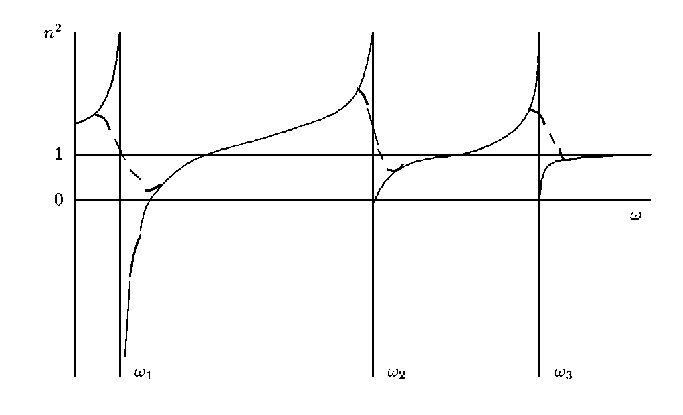
\includegraphics[scale=0.9]{Ris/ris_eps/ris3_04.eps}}}

\risp{4}{Кривая дисперсии при наличии нескольких полос поглощения}
\end{figure}

Так как измерения
показателя преломления (рефракции) обычно производятся в
прозрачной, т.е. достаточно удаленной от собственных полос
поглощения спектральной области, можно пользоваться формулой, в
которой не учитывается затухание. Окончательно получаем:
$${n^2-1\over n^2+2}={4\pi\over3}N_1\sum_{i}{f_i\over
\omega_i^2-\omega^2},\noq$$
$$R={n^2-1\over n^2+2}{M\over\rho}={4\pi\over3}N_A{e^2\over
m}\sum_{i}{f_i\over \omega_i^2-\omega^2}.\eqno (3.40a)$$

\subzag{О квантовомеханической теории дисперсии}

Выше мы ограничились краткими сведениями по классической теории дисперсии.
Наиболее важным и общим результатом классической электронной
теории дисперсии является установление тесной связи между
дисперсией и поглощением света. Недостатком классической теории
является формальный характер введения сил осцилляторов $f_i$,
характеризующих степень участия электрона в данном колебании.

Обычный метод рассмотрения взаимодействия вещества со светом
состоит в квантовании частиц вещества, но сохранении для
электромагнитного поля света классических выражений. Это возможно
на основании принципа соответствия. При квантовании атома или
молекулы мы должны отказаться от классической модели
гармонического осциллятора. Однако, в квантовомеханической теории
излучения, исходящей из комбинационного принципа, связывающего
частоту испускаемой или поглощаемой световой волны с разностью
энергий комбинирующих уровней:
$$\hbar \omega_{mn}=E_m-E_n.\noq$$
Интенсивность соответствующей спектральной линии испускания или
поглощения выражается через вероятность перехода $m\leftrightarrow
n$. Большей частью в оптике приходится встречаться с
квантовомеханическими переходами дипольного характера. Их
вероятности определяются матричными элементами электрического
дипольного момента:
$$\vec p_{mn}=\int\psi_m^*\vec p\psi_nd\tau=e\int\psi_m^*\vec
r\psi_nd\tau,\noq$$ и интенсивность, точнее --- величина обще
энергии, излучаемой в единицу времени при переходе
$m\leftrightarrow n$ дается уравнением:
$${dW\over dt}={4\over3}{\omega^4_{mn}\over c^3}|\vec p_{mn}|^2.\noq$$

Решая волновое уравнение для гармонического осциллятора, мы
находим собственные функции $\psi_n$ и, следовательно, приобретаем
возможность вычисления матричных элементов \eqn{43}. Расчет
показывает, что матричный элемент отличен от нуля только для таких
переходов, при которых квантовое число $n$ меняется на $\pm 1$.
Тем самым:
$$\omega_{mn}=\omega_{n+1,n}={1\over\hbar}(E_{n+1}-E_n)={\hbar \omega\over\hbar}
\left(n+{3\over2}-n-{1\over2}\right)=\omega,\noq$$ т.е. частота,
излучаемая (или поглощаемая) гармоническим осциллятором, согласно
квантовой механике, совпадает с его классической собственной
частотой колебаний. Квантовомеханическое поведение гармонического
осциллятора не отличается в этом смысле от классического.
Величина, которая в квантовой механике совпадает с классической
собственной частотой колебаний осциллятора, не зависит от
амплитуды его колебаний. << Квантуется>> именно амплитуда.
Указанным свойством совпадения результатов квантовомеханического и
классического рассмотрения процессов испускания и поглощения света
обладает только гармонический осциллятор. Его частота не
квантуется.

Что касается выражений \eqn{43} и \eqn{44}, характеризующих
интенсивность излучения, интенсивность спектральной линии, то эти
соотношения ограничены случаем излучения электрического диполя.
Именно электрическое дипольное излучение и поглощение обладает
наибольшей интенсивностью и именно с ним приходится иметь дело в
большинстве оптических явлений. Легко видеть, что формула \eqn{43}
аналогична классическому выражению \eqn{10} для общей энергии,
излучаемой гармонически-колеблющимся электрическим диполем. Эти
формулы совпадут, если принять:
\begin{plain}$$\eqalign{
&\omega_0=\omega_{mn},\cr &(\overline{p^2})_{\rm \hbox{классич}.}=2|\vec
p_{mn}|^2. }\noq$$ 
\end{plain} Множитель 2 возникает вследствие возможности
двух независимых направлений поляризации излучения
квантовомеханической системы, перпендикулярных к лучу. Таким
образом, имеется прямое соответствие между излучением, относящимся
к переходу $m\rightarrow n$ и излучением некоторого осциллятора,
характеризуемого условиями \eqn{45}.

Таким образом, при характеристике оптических свойств атома или
молекулы (ограничиваясь рассмотрением дипольных моментов) приходим
к выводу о соответствии классических и квантовомеханических
выражений.

Классическому осциллятору с частотой $\omega_0$ и силой
осциллятора $f$, определяющей интенсивность линии в спектре,
соответствует матрица частот:
$$\omega_{mn}={1\over\hbar}(E_m-E_n); \eqno (3.41)$$
$$\left|\matrix{
0&\omega_{12}&\cdots&\omega_{1n}&\cdots\cr
\omega_{21}&0&\cdots&\omega_{2n}&\cdots\cr
\cdots&\cdots&\cdots&\cdots&\cdots\cr
\omega_{m1}&\omega_{m2}&\cdots&\omega_{mn}&\cdots\cr
\cdots&\cdots&\cdots&\cdots&\cdots\cr }\right|,$$ и матрица <<
амплитуд>>\ электрического момента:
$$\left|\matrix{
p_{11}&p_{12}&\cdots&p_{1n}&\cdots\cr
p_{21}&p_{22}&\cdots&\omega_{2n}&\cdots\cr
\cdots&\cdots&\cdots&\cdots&\cdots\cr
p_{m1}&p_{m2}&\cdots&p_{mn}&\cdots\cr
\cdots&\cdots&\cdots&\cdots&\cdots\cr }\right|.$$ Диагональные
элементы матрицы $p_{mn}(t)$ не зависят от времени, так как, по
определению, $\omega_{nn}=0$. При этом интенсивности (>> силы
осцилляторов<<) выражаются через элементы матрицы \eqn{48}
следующим образом:
$$f_{nk}={2m|p_{nk}|^2\omega_{kn}\over3e^2\hbar}.\noq$$
Различие в точках зрения проявляется в частном случае
одноэлектронной системы (орбитальная модель атома водорода) в том,
что согласно классической теории, в такой системе имеется один
электрон с $f=1$ и определенной частотой $\omega_0$ и,
следовательно, поляризуемость может быть выражена одночленной
дисперсионной формулой, а согласно квантовой механике, уже в такой
системе мы имеем целый набор осцилляторов, характеризуемый
матрицами \eqn{47} и \eqn{48}, и, следовательно, дисперсионная
формула должна, по аналогии с классической формулой \eqn{39},
выражаться суммой. В общем случае:
$$\alpha={e^2\over m}\sum_n\sum_k \omega_n{f_{nk}\over
\omega^2_{nk}-\omega^2}.\noq$$ Здесь $\omega_n$ --- вероятность
того, что система находится в состоянии с энергией $E_n$. Можем
принять по Больцману:
$$\omega_n=e^{-{E_n\over kT}}.$$
Так как энергия возбуждения электронов, как правило, значительно
больше $kT$, мы можем практически отвлечься от
электронно-возбужденных состояний и, отсчитывая энергию от
основного уровня с $n=0$, положить $\omega_0=1$. Следовательно:
$$\alpha={e^2\over m}\sum_{k}{f_{0k}\over \omega^2_{0k}-\omega^2}.\eqno
(3.47a)$$ Существенно новым результатом квантовомеханического
рассмотрения по сравнению с классической теорией является
объяснение отрицательной дисперсии. В классической теории все
величины $f_i>0$. В квантовой теории такого ограничения нет. Если
мы имеем дело с электронно-возбужденным состоянием с энергией
$E_n$, то некоторые из $f_{nk}$ могут быть отрицательны, а именно
те, для которых $\omega_{kn}<0 (E_k<E_n)$. При этом ход дисперсии
может стать обратным обычному (рис. 3.5). Явление отрицательной
дисперсии действительно удается наблюдать при определенных
условиях.

\begin{figure}[tbp]
\centerline{\hbox{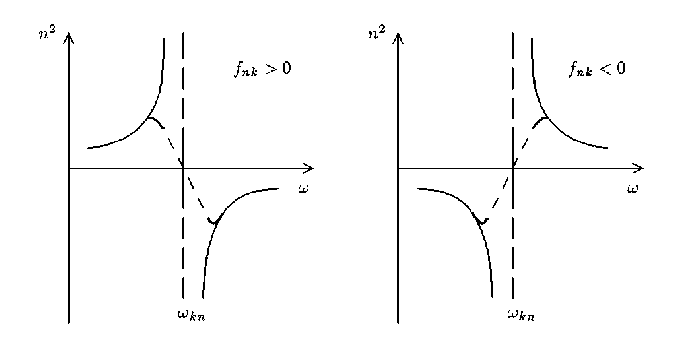
\includegraphics[scale=0.9]{Ris/ris_eps/ris3_05.eps}}}

\risp{5}{Положительная и отрицательная дисперсия}
\end{figure}

Теоретическое вычисление
$f_{nk}$ требует знания волновых функций $\psi_n,\ \psi_k$
системы. В настоящее время такие расчеты пока невозможны. Величины
$f_{nk}$ определяются из опыта, который может с полным правом быть
истолкован при помощи классических соображений. Существует два
замечательных экспериментальных метода исследования дисперсионных
явлений, дающих возможность с высокой точностью определить ход
дисперсии и силы осцилляторов. Это метод крюков Д. С.
Рождественского и дифракционный метод И. В. Обреимова. Описание
данных методов можно найти в курсе << Молекулярная оптика>>\ М.
В. Волькенштейна и в сборнике Д. С. Рождественского << Природа
света>>.

Как показывает квантовая механика, величины $f_{nk}$ удовлетворяют
условию суммы, которое может рассматриваться, как аналогичное
\eqn{39}. Квантовая механика показывает, что для каждого
электрона, находящегося в состоянии, характеризуемом квантовым
числом $n$, имеет место условие:
$$\sum_{k}f_{nk}=1;\noq$$
$$\sum\limits_{\rm \hbox{по\ всем\
электронам}}\left(\sum_{k}f_{nk}\right)=Z.\eqno (3.48a)$$ Здесь
суммирование распространяется по всем электронам, участвующим в
процессе.

Таким образом, сопоставление данных классической и
квантовомеханической теории дисперсии показывает, что решая
проблемы, связанные с электрическим дипольным излучением и
поглощением света, мы вправе пользоваться простой классической
моделью гармонического осциллятора. Численные значения
фигурирующих в наших формулах величин --- частот и сил
осцилляторов --- могут быть найдены теоретически только в
квантовой механике, поскольку атом или молекула являются
микрообъектами, недоступными рассмотрению в рамках классической
теории. Однако ввиду практической невозможности решения волнового
уравнения для многоэлектронной системы, приходится пользоваться
опытными значениями частот и интенсивностей, причем можно
трактовать их классически. Следовательно, теория явлений, так или
иначе связанных с излучением и поглощением --- с дисперсией света
в веществе, может разрабатываться в настоящее время как
классическая полуэмпирическая теория, в основу которой положена
модель гармонического осциллятора.

\subzag{Дисперсия и рефракция} 

Рассмотрим опытные данные, характеризующие ход дисперсии в некоторых чистых
веществах. Наблюдаемый ход дисперсии принято выражать
эмпирическими формулами, в которых обычно удается ограничиться
небольшим числом членов. Одночленной формулой можно пользоваться в
тех случаях, когда все полосы поглощения, кроме ближайшей,
обладающей частотой $\omega_0$, либо лежат в далекой области
$\omega_i\gg \omega$, либо обладают малыми силами осцилляторов
$f_i$:
$$n\cong1+2N_1{e^2\over m}{f\over \omega_0^2-\omega^2}.\noq$$
Экстраполируя значение рефракции к бесконечно большим длинам волн,
находим среднюю статическую поляризуемость $\alpha^{\circ}$. Имеем
для оптической поляризуемости формулу:
$$\alpha_{\rm \hbox{опт.}}={e^2\over m}\sum_{i}{f_i\over \omega_i^2-\omega^2},\noq$$
и, положив $\omega=0$, получаем среднюю статическую
поляризуемость:
$$\alpha^{\circ}={e^2\over m}\sum_{i}{f_i\over \omega_i^2}.\noq$$
Величины $\alpha_{\rm \hbox{опт.}}$ и $\alpha^{\circ}$ тем ближе друг к
другу, чем дальше лежит полоса поглощения $\omega_i$ от той
области спектра, в которой мы проводим измерения. Рассмотрим
пример. Допустим, что длина волны падающего света
$\lambda=5000\angst$, а собственная полоса поглощения лежит при
$\lambda_0=1000\angst$. Тогда величина
$${1\over
\omega_0^2-\omega^2}={1\over4\pi^2c^2}{\lambda_0^2\lambda^2\over\lambda^2-\lambda_0^2}=
{1\over4\pi^2c^2}\cdot1,04\cdot10^{6}\angst^2$$ всего на 4\%
отличается от величины
$${1\over
\omega_0^2}={1\over4\pi^2c^2}\lambda^2_0={1\over4\pi^2c^2}\cdot1,00\cdot10^6\angst^2.$$
Напротив, если полоса поглощения лежит в области, близкой к
области измерения, различие между оптической и статической
поляризуемостью значительно. Допустим, что по-прежнему
$\lambda=5000\angst$, но $\lambda_0=4000\angst$. Имеем:
$${1\over{\omega_0^2-\omega^2}}={1\over4\pi^2c^2}\cdot44,4\cdot10^6\angst^2,$$
$${1\over \omega_0^2}={1\over4\pi^2c^2}\cdot16\cdot10^6\angst^2.$$
Расхождение в этом случае приближается к 300\%.

Отсюда следует, что для веществ, обладающих только полосами
поглощения, расположенными в далекой ультрафиолетовой области
спектра, практически допустимо отождествление статической
поляризуемости с оптической в видимом спектре. Здесь
следовательно:
$$n^2\cong\varepsilon.\noq$$
Такого рода спектрами обладают, например, предельные углеводороды.
Заметные расхождения не только между $n^2$ и $\varepsilon$, но и
$n_{\infty}^2$ и $\varepsilon$ у $\rm CO_2$, $\rm CO$, $\rm CH_4$,
$\rm C_2H_4$, и факт, что в действительности почти
всегда $n^2_{\infty}<\varepsilon$ связаны с наличием атомной
рефракции.

Для веществ, обладающих полосами поглощения в близкой
ультрафиолетовой и видимой области, отождествление статической и
оптической поляризуемости невозможно. В этих случаях мы
непосредственно сталкиваемся с аномальной дисперсией. Приближение
к собственной полосе поглощения в области аномальной дисперсии
резко повышает поляризуемость (показатель преломления) вещества.

Выше указывалось, что чередование двойных и единичных $C-C$ связей
приводит к нарушению аддитивности рефракции, к экзальтации.
Очевидно, что само значение экзальтации должно зависеть от длины
волны света. Поэтому важно выяснить, определяется ли аномальное
повышение рефракции действительным следствием специфической
структуры молекулы, или мы просто попадаем, измеряя рефракцию, в
область длин волн, близкую к собственным полосам поглощения --- в
область аномальной дисперсии.

Рассмотрим случай паранитроанилина:

%\begin{figure}[tbp]
\centerline{\hbox{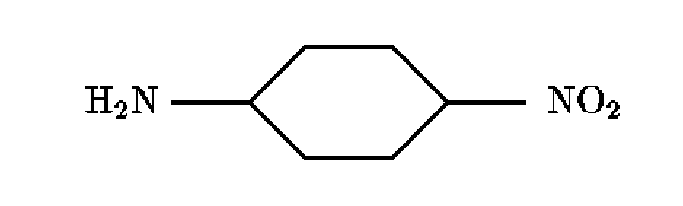
\includegraphics[scale=0.5]{Ris/ris_eps/ris3_05a.eps}}}
%\end{figure}

Измерение рефракции при $\lambda=4358\angst$ (синяя
линия ртутного спектра) дает весьма высокое значение экзальтации,
равное $14,85\rm\ \hbox{см}^{3}$. Однако это значение быстро уменьшается
с увеличением длины волны света. Имеем:
\begin{plain}$$\eqalign{
\Delta R_{4358}=&14,85\ {\rm \hbox{см}^{3}},\cr \Delta R_{5460}=&7,01\
{\rm \hbox{см}^{3}},\cr \Delta R_{5790}=&6,40\ {\rm \hbox{см}^{3}},\cr \Delta
R_{6707}=&5,23\ {\rm \hbox{см}^{3}},\cr \Delta R_{\infty}=&2,70\ {\rm
\hbox{см}^{3}} }$$ \end{plain}
очевидно, что освещая п-нитроанилин светом с
$\lambda=4358\angst$, мы попадаем в область, близкую к аномальной
дисперсии. В самом деле, п-нитроанилин имеет полосу поглощения при
$\lambda=3200-4050\angst$ (в зависимости от растворителя).
Истинный физический смысл имеет экзальтация статическая ---
экстраполированная к нулевой частоте световой волны. Эти
обстоятельства всегда следует иметь в виду при оптической
характеристике вещества.

Из изложенного выше очевидно, что подлинное физическое содержание
аддитивности или неаддитивности рефракции может быть установлено
лишь на основе спектроскопических данных. Поляризуемость молекулы
есть специфическое проявление ее спектра --- она непосредственно
определяется совокупностью энергетических уровней и вероятностями
переходов между ними.

Все органические соединения обладают полосами поглощения, лежащими
в далекой ультрафиолетовой шумановской области спектра. Эта
область простирается от 1800 \angst\ в сторону меньших длин волн.
Если других полс поглощения нет (например, насыщенные
углеводороды), то рефракция аддитивна. Неаддитивные соединения
--- это соединения, содержащие так называемые хромофорные группы:
сопряженные связи, ароматические кольца, группы $\rm >C=O$, $\rm
-C\equiv C-$, $\rm -N\equiv N-$, $-NO_2$ и т.д.

Наличие этих групп определяет цветность органических соединений
--- сдвиг полос поглощения в длинноволновую область. Тем самым,
хромофорные группы определяют наличие экзальтации рефракций у
соответствующих соединений.

В практическом и принципиальном отношении весьма важен вопрос о
влиянии межмолекулярного взаимодействия на рефракцию и дисперсию
вещества. Во-первых, существенно прямое влияние межмолекулярных
сил на спектр и, тем самым, на поляризуемость. Во-вторых, не
следует забывать, что в выражении для рефракции фигурирует средняя
поляризуемость, получаемая из усреднения по всем равновероятным
ориентациям молекулярного хаоса. Однако взаимная ориентация
молекул, вызванная межмолекулярными силами, может привести к
изменению статистики и, следовательно, к изменению значения
поляризуемости (здесь нельзя уже использовать поляризуемость,
получаемую при усреднении по всем равновероятным ориентациям).

\subzag{Аналитические применения дисперсионной формулы}

Перейдем теперь к некоторым аналитическим применениям
дисперсионной формулы. Дисперсия является важным аналитическим
признаком для вещества. Можно характеризовать вещество величиной
молекулярной дисперсии --- разности молекулярных рефракций для
определенных длин волн:
$$D_{12}=R_{\lambda_1}-R_{\lambda_2}={M\over\rho}\left\{
{n_1^2-1\over n_1^2+2}-{n_2^2-1\over n_2^2+2}\right\}.\noq$$
Величины такого типа также должны обладать аддитивностью в тех случаях,
когда имеет место аддитивность рефракций. Имеем, следовательно:
$$D_{12}=\sum_i(D_{12})_i.\noq$$
В ряде случаев сопоставление наряду с молекулярными рефракциями
также и молекулярных дисперсий позволяет повысить точность
структурного анализа вещества.

Наличие дисперсионной зависимости позволяет, исходя из
аддитивности молекулярных рефракций, анализировать
многокомпонентные смеси. Рассмотрим случай трехкомпонентной смеси.
Имеем уравнения:
\begin{plain}
$$\eqalign{
&c_1+c_2+c_3=1,\cr &R_1c_1+R_2c_2+R_3c_3=R,\cr
&R'_1c_1+R'_2c_2+R'_3c_3=R', }\noq$$ 
\end{plain}
где $c_1$, $c_2$, $c_3$ ---
молярные доли трех компонентов. Здесь величины $R_1$, $R_2$, $R_3$,
$R$ относятся к длине волны $\lambda_1$, а $R'_1$, $R'_2$, $R'_3$,
$R'$ --- к длине волны $\lambda_2$. Второе и третье уравнения
эквивалентны:
$$D_{12}=R'-R=c_1(R'_1-R_1)+c_2(R'_2-R_2)+c_3(R'_3-R_3)=\sum_{i}c_i
D_{12_i}.\noq$$ Последнее уравнение выражает аддитивность
молекулярной дисперсии в смесях.

Решения системы уравнений \eqn{58} имеют вид:
$$c_1={\Delta1\over \Delta},\ c_2={\Delta2\over\Delta},\
c_3={\Delta3\over\Delta},\noq$$
$$\Delta=\left|\matrix{
R_2-R_1,&R_3-R_2\cr R'_2-R'_1,&R'_3-R'_2\cr }\right|;\hskip 3mm
\Delta_1=\left|\matrix{ R_2-R,&R_3-R_2\cr R'_2-R',&R'_3-R'_2\cr
}\right|;$$
$$\Delta_2=\left|\matrix{
R-R_1,&R_3-R\cr R'-R'_1,&R'_3-R'\cr }\right|;\hskip 3mm
\Delta_3=\left|\matrix{ R_2-R_1,&R-R_2\cr R'_2-R'_1,&R'-R'_2\cr
}\right|.$$ Согласно И. В. Обремову, можно достичь по этому методу
точности определения состава трехкомпонентной смеси порядка 1\%.

Непосредственно значения молекулярной дисперсии применяются для
определения содержания ароматических соединений в смесях
углеводородов. Удобно характеризовать дисперсию вещества
величиной:
$$\delta={n_1-n_2\over n_3-1}\cdot10^3.\noq$$
Здесь $n_1$, $n_2$, $n_3$ --- показатели преломления, измеренные
при длинах волн $\lambda_1=4861\angst$, $\lambda_2=6563\angst$,
$\lambda_3=5893\angst$. Измерения проводятся для всех веществ при
одной и той же температуре $T=20^{\circ}$; $10^3$ --- множитель,
вводимый для удобства.

Обращают на себя внимание значительно большие величины
относительных дисперсий $\delta$ для ароматических соединений, а
также большая чувствительность этих величин к структуре молекулы.
Эти факты связаны с наличием у ароматических соединений полос
поглощения в близкой ультрафиолетовой части спектра, в то время
как у насыщенных соединений полосы располагаются в далекой
области. На основании такого резкого отличия $\delta_{\rm
\hbox{аромат}.}$ от $\delta_{\rm \hbox{алифат}.}$ можно определять концентрацию
ароматики в смеси с насыщенными углеводородами, пользуясь простой
формулой:
$$c=K(\delta_{\rm \hbox{смеси}}-\delta_{\rm \hbox{алифат}.}),\noq$$
где константа $K$ равна:
$$K={100\over \delta_{\rm \hbox{аромат}.}-\delta_{\rm \hbox{алифат}.}}.$$
Среднее значение по большинству алифатических соединений
$\delta\approx17,5$. Имеем для бензола (и в общем случае):
$$c=6,92(\delta_{\rm \hbox{смеси}}-17,5),$$
для толуола:
$$c=6,75(\delta_{\rm \hbox{смеси}}-17,5),$$
и т.д.

При практическом пользовании рефрактометром Аббе, точность таких
определений достигает 1\%. Б. В. Иоффе показал, что при работе на
рефрактометре Пульфриха удобнее пользоваться величиной
$$\delta'={n_1-n_2\over n_2-1}\cdot10^3.\noq$$
$\delta'$ мало отличается от $\delta$. В других работах
рекомендуют применять не относительную, а удельную дисперсию:
$$\delta''={n_{\beta}-n_{\alpha}\over\rho}\cdot10^4.\noq$$
Здесь $\rho$ --- плотность, $n_{\beta}$ --- показатель преломления
для $\lambda_{{\rm H}_{\beta}}=4861\angst$, $n_{\alpha}$ --- для
$\lambda_{{\rm H}_{\beta}}=6593\angst$. Величина $\delta''$ также
аддитивна. Для насыщенных углеводородов $\delta''$ в среднем равна
99; для ароматических $\delta''$ значительно выше (бензол 190,
толуол 185, ксилол 180 и т.д.).

\subzag{Цветность органических соединений}

Это явление напрямую связано с электронными спектрами молекул --- со спектрами
поглощения, определяемыми электронными переходами в сложных
молекулах. Все органические соединения обладают полосами
поглощения в далекой ультрафиолетовой области спектра (в так
называемой вакуумной области $\lambda\leq1800\angst$). Насыщенные
углеводороды имеют полосы поглощения только в вакуумной области.
Их производные, а также соединения с сопряженными связями и просто
соединения, имеющие производные, а также соединения с сопряженными
связями и просто соединения, имеющие $\pi$-электроны, имеют кроме
того, полосы поглощения и в длинноволновой области спектра.

Эти полосы поглощения определяются электронными переходами в
сложных молекулах. Только часть электронов --- внешние или
валентные электроны --- обобществлены в химических связях и могут
рассматриваться как молекулярные. До известной степени каждый атом
сохраняет в молекуле свою индивидуальность благодаря тому, что
около его ядра удерживаются внутренние электроны. Энергетические
переходы внутренних электронов в молекуле подобны тем, которые
осуществляются в отдельных атомах. Именно эти переходы
локализуются в вакуумной области спектра. Полосы поглощения,
соответствующие таким переходам, должны быть характеристичны.

Но помимо таких переходов в молекуле существуют переходы внутри
валентной электронной оболочки. Часть электронов (внешние или
валентные электроны) обобществлены в химических связях. Их можно
назвать << молекулярными электронами>>. Переходы, относящиеся к
валентной оболочке, связаны с $\pi$-электронами и
$\sigma$-электронами.

Если система без сопряженных связей, то эти переходы могут также
быть характеристичными и определять появление полос как в
вакуумной, так и в более близкой части спектра.

Строгой характеристичности, однако, нет, так как возможно взаимное
влияние связей, сказывающееся на состоянии электронной оболочки, а
значит и на спектре поглощения молекулы.

Аддитивность молекулярной рефракции, установленная на опыте для
соединений без сопряженных связей, связана с аддитивностью $f_i$ и
$\omega_i$ для внутренних атомных электронов, энергетическим
переходам которых соответствует особенно большие $f_i$. Отсутствие
строгой характеристичности у переходов молекулярных электронов не
препятствует аддитивности поляризуемости, если силы осцилляторов
атомных переходов и частоты колебаний молекулярных электронов
далеки от частоты падающего света. Это означает, что
соответствующие члены в сумме $\sum_{i}{f_i\over
\omega_i^2-\omega^2}$ в формуле \eqn{41a} малы по сравнению с
членами, определяемыми внутренними электронами.

Обобществленные в молекуле подвижные $\pi$-электроны определяют
наряду с коротковолновыми также и длинноволновые полосы
поглощения, попадающие в близкий ультрафиолет и видимую часть
спектра. Проблема цветности органических соединений сводится к
рассмотрению свойств подвижных $\pi$-электронов.

Основные факты, позволяющие связать спектр поглощения ---
цветность вещества --- с его строением, были установлены химиками
задолго до того, как проблема происхождения электронных спектров
могла быть вообще поставлена в физической науке. Еще в 1876 году
Витт пришел к заключению, что цветность органических соединений
связана с присутствием в них определенных групп и связей,
названных им хромофорами. В таблице 3.1 приведены некоторые
важнейшие хромофорные группы.

Наряду с хромофорами в окрашенных соединениях имеются ауксохромы
--- группы, которые в результате взаимодействия с хромофорами
углубляют цвет соединения и определяют смещение полос поглощения к
более длинным волнам.

Эффект углубления окраски называется батохромным, а эффект
увеличения интенсивности полосы поглощения --- гиперохромным.
Обратные эффекты носят соответственно названия гипсохромного и
гипохромного.

Ауксохромы могут быть << положительными>>\ --- они углубляют
окраску (т.е. усиливают интенсивность полос поглощения и
определяют их смещение к более длинным волнам) у катионов
красителей. Типичные представители этой группы: $\rm OH$, $\rm
OR$, $\rm NH_2$, $\rm NHR$, $\rm NR_2$ (R - алифатический
радикал), см. рис. 3.5а.
\begin{figure}[tbp]
\centerline{\hbox{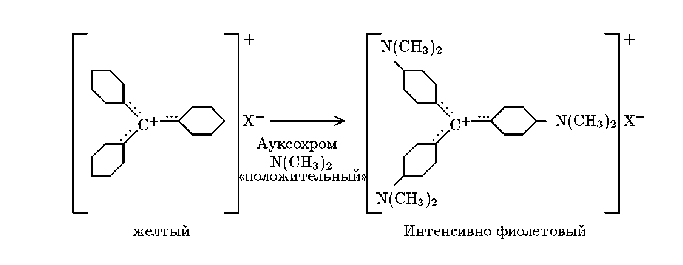
\includegraphics[scale=0.9]{Ris/ris_eps/ris3_05b.eps}}}
\risp{5а}{Реакция на << положительный>> ауксохром}
\end{figure}

Если окраска определяется анионом, то
роль << отрицательных ауксохромов>> играют другие группы: $\rm
NO$, $\rm NO_2$, $\rm SO_2$, $\rm -N=N-$ и др., см. рис. 3.5б.

\begin{figure}[tbp]
\centerline{\hbox{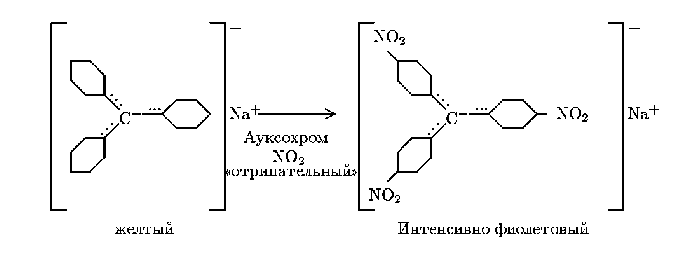
\includegraphics[scale=0.9]{Ris/ris_eps/ris3_05c.eps}}}
\risp{5б}{Реакция на << отрицательный>> ауксохром}
\end{figure}


\begin{figure}[tbp]
\tabp{1}{Органические хромофоры}
\vskip 5 mm
\centerline{\hbox{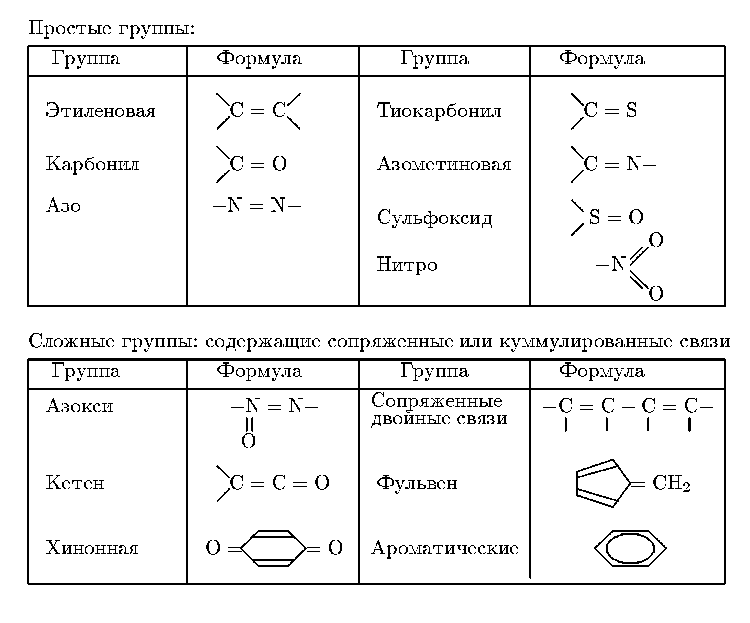
\includegraphics[scale=0.9]{Ris/ris_eps/ris3_05d.eps}}}
\end{figure}

Связь между цветностью, т.е. положением полосы
поглощения, и химическим строением сложных молекул --- одна из
важных проблем теоретической химии. Следуя монографии А. Н.
Теренина (см. рис 3.6), показывающей соотношение между положением
полосы поглощения в видимом спектре и цветом пропускания ---
окраской вещества, рассмотрим особенности строения красителей
более подробно.

\begin{figure}[tbp]
\centerline{\hbox{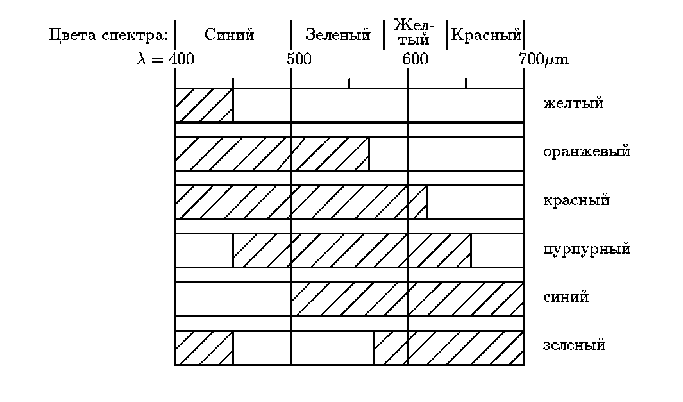
\includegraphics[scale=1.0]{Ris/ris_eps/ris3_06.eps}}}

\risp{6}{Положение полос поглощения и окраска (по А. Н. Теренину)}
\end{figure}

Большинство сильно окрашенных органических соединений содержит
ненасыщенные циклические группировки с обобществленными
$\pi$-электронами, например:

\vskip 3mm
\centerline{\hbox{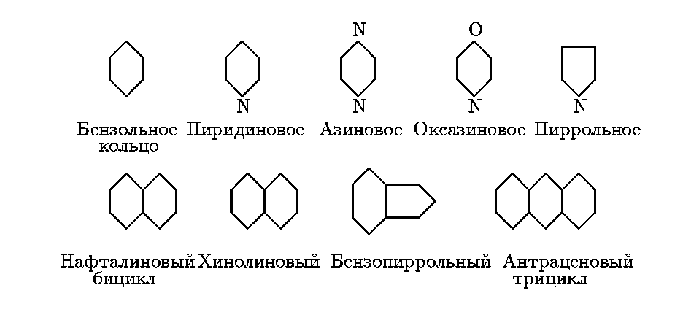
\includegraphics[scale=1.0]{Ris/ris_eps/ris3_06a.eps}}}

\leftskip 0cm В молекуле эти циклы связаны друг с другом или через
посредство некоторого центрального атома (например,
трифенилметановые красители), или цепочками сопряженных связей,
как например:
\begin{plain}
$$\eqalign{
&{\rm -N=N-}\hskip 7mm{\rm -CH=CH-CH=CH-}\hskip 7mm{\rm
-CH=N-CH=N-}\cr &{\rm \hbox{азогруппа}}\hskip 10mm{\rm \hbox{полиметиновая\
цепь}}\hskip 14mm{\rm \hbox{азометиновая\ цепь}} }$$
\end{plain}
Таким образом,
красители представляют собой сложные системы сопряженных
$\pi$-связей, взаимодействующих с циклическими системами
$\pi$-связей ароматического типа. Сопряжение определяет плоское
строение молекул красителей. Большинство красителей представлено
положительными и отрицательными ионами. Необходимо подчеркнуть,
что многие красители обладают свойствами индикаторов
--- меняют свой цвет при изменении концентрации водородных ионов
в окружающей среде. Например, в кислой среде метилоранж имеет
красный цвет, а в щелочной --- желтый. Фенолфталеин, относящийся к
группе ксантеновых красителей, имеет в щелочной среде ярко
пурпурный цвет, а в кислой среде --- бесцветен. Иными словами,
положение полосы поглощения существенным образом зависит от заряда
иона красителя. Способность молекулы красителя образовывать
положительные и отрицательные ионы определяется ионогенными
свойствами ауксохромных групп. Такие группы, как $\rm NH$ или $\rm
HR_2$, характеризуются основными свойствами, группы $\rm OH$ (в
феноле) и $\rm HSO_3$ --- кислыми.

Непосредственная зависимость цветности от сопряжения $\pi$-связей
в красителях может быть иллюстрирована тем фактом, что при
гидрировании некоторых красителей, при уничтожении $\pi$-связей
получаются бесцветные соединения.

Таким образом, строение молекулы красителя обычно характеризуется
двумя важнейшими факторами: сопряжением $\pi$-связей и ионизацией.
Первый фактор практически обязателен для того, чтобы органическое
соединение обладало интенсивной полосой поглощения в видимой
области. Второй фактор может и не иметь места, хотя всегда
способствует появлению окраски.
